
\documentclass{beamer}
\usepackage{graphicx}


%Global Background must be put in preamble


\usetheme{Madrid}

\title{COP 290}

\subtitle{Designing Documentation}

\author{Ayushya Raj \and Nitin Rathor \and Ankush Phulia}

\institute[IIT Delhi] 
{
  Department of Computer Science\\
  IIT Delhi}

\subject{COP 290}



\begin{document}

{\usebackgroundtemplate%
{
\includegraphics[width=\paperwidth,height=\paperheight]{back.png}}
\begin{frame}
  \titlepage
\end{frame}
}
{\usebackgroundtemplate%
{
\includegraphics[width=\paperwidth,height=\paperheight]{back.png}}
\begin{frame}{Application Description}{}
  \begin{itemize}
  \item {
   A user-friendly application to enable someone to explore his moodleplus account maintained at the given server.
  }
  \item {
    Divided into activities with some fragments along with various design layouts and resources for various part of the user interface.
  }
  \item {
    Followed by login activity there is main activity containing drawer with an expandablelist view containing headers like grades courses and notification.
  }
  \item{
  Volley network library used (as encouraged) to send and receive data from the server, if all the details are properly provided.
  }
  \end{itemize}
\end{frame}
}
{\usebackgroundtemplate%
{
\includegraphics[width=\paperwidth,height=\paperheight]{back.png}}

\begin{frame}{Application Features}
  \begin{itemize}
  \item {
    Session handler can remember multiple username and passwords and given a username password is set automatically if it was saved.
  }
  \item {   
    In the dashboard there is a calander so  one can have a quick view of important dates and also enabling one to mark important dates there.
  }
  \item {
    Drawer contain group headers like Overview,Grades,Notifications and Courses enabling faster acces to data with a friendly UI.
  }
  \item {
    Course information is displayed in a tab layout view for the above mentioned reasons from where the user can freely navigate to tabs like threads overview etc.
  }
  \item {
    For many error conditions toast are made to appear with related information.
  }
  \end{itemize}
\end{frame}
}
{\usebackgroundtemplate%
{
\includegraphics[width=\paperwidth,height=\paperheight]{back.png}}

\begin{frame}{High Level Functions Used }
\begin{block}{Text-Watcher Methods}
To autofill the password edit text if the password corresponding to that username was remembered.
\end{block}
\begin{block}{populate()}
To populate data related to expandable list 
\end{block}
\begin{block}{On Click Methods}
For buttons which involve navigation, checking and sending requests to servers.
\end{block}
\begin{block}{Various Methods for Request Queue}
A separate class used to implement a global request queue in order to avoid creating a new one on every button click.
\end{block}


\end{frame}
}

\begin{frame}{How to use the app ? }
    \begin{enumerate}
        \item  
        \item 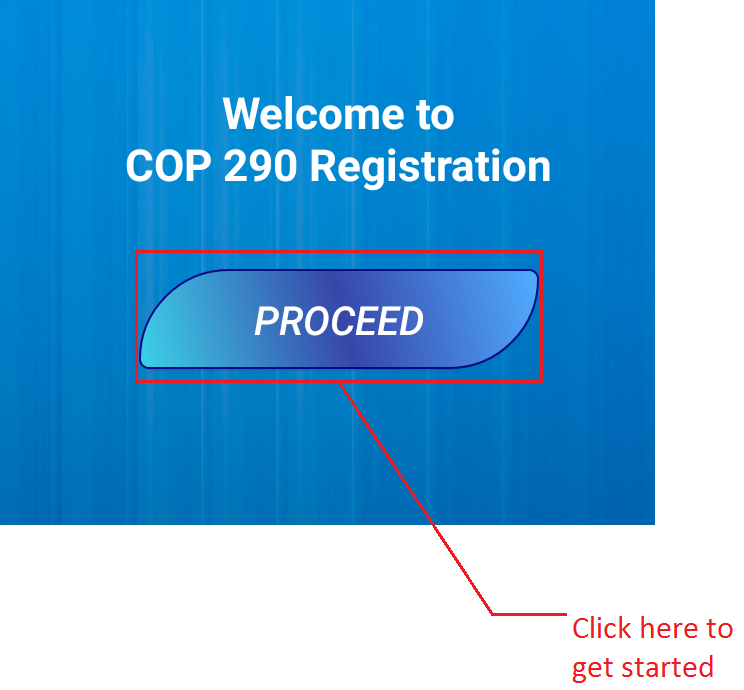
\includegraphics[scale = 0.153]{img1.png}        
        \item 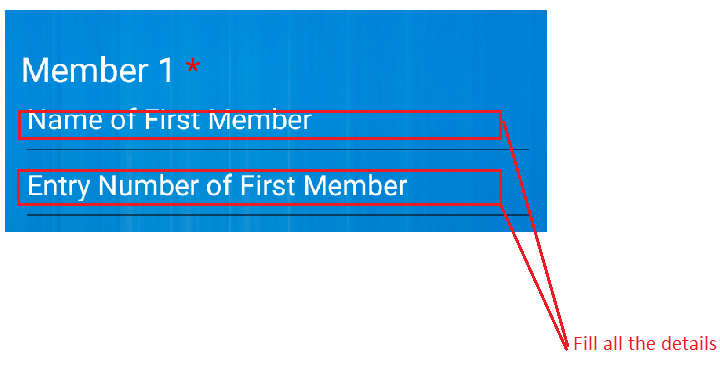
\includegraphics[scale = 0.25]{img2.png}
        \item 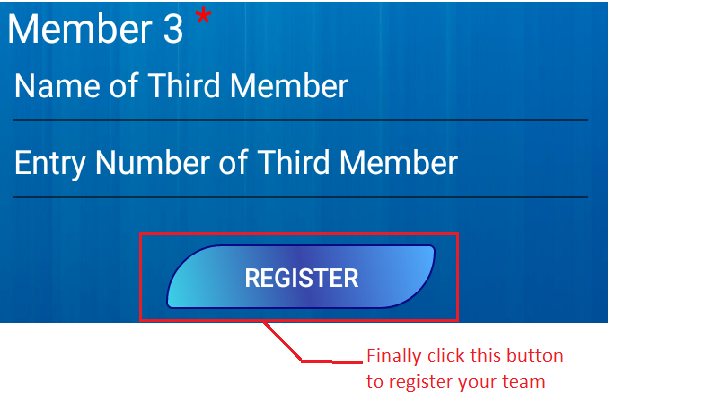
\includegraphics[scale = 0.225]{img3.png}
    \end{enumerate}
    
    
    
    
\end{frame}

{\usebackgroundtemplate%
{
\includegraphics[width=\paperwidth,height=\paperheight]{back.png}}

\begin{frame}{References}
    
    \begin{itemize}
        \item {Basic Reference:\\developer.android.com/training/}
        \item {Volley References :\\ developer.android.com, androidhive.info}
        \item {Icon Images and Backgrounds:\\ tradefair.omaheke.com, tophdimg.com }
        \item {Miscellaneous methods and troubleshooting :\\ Android Documentation, Stack Overflow}
    \end{itemize}
    
\end{frame}
}

\end{document}


